\documentclass[aps,prb,superscriptaddress,nofootinbib]{revtex4}
\usepackage{amsfonts}
\usepackage{amsmath}
\usepackage{amssymb}
\usepackage{graphicx}
\usepackage{caption}
\usepackage{bm}
\usepackage{bbm}
\usepackage{cancel}
\usepackage{color}
\usepackage{mathrsfs}
\usepackage[colorlinks,bookmarks=true,citecolor=blue,linkcolor=red,urlcolor=blue]{hyperref}
\usepackage{appendix}
\usepackage{float}
\usepackage{array}
\usepackage{booktabs}
\setlength{\parindent}{10 pt}
\setlength{\parskip}{2 pt}
\setcounter{MaxMatrixCols}{30}
\bibliographystyle{apsrev}

\newcommand{\normord}[1]{{:\mathrel{#1}:}}
\def\tbs{\textbackslash}
\def \tr{\operatorname{tr}}
\def \Tr{\operatorname{Tr}}


\begin{document}
\title{Quantization of Quantum Fields}
\author{Jie Ren}



\maketitle

\tableofcontents




\section{Quantization of Klein-Gordon Field}

In this section, we discuss the quantization of the Klein-Gordon field
\begin{equation}
	\mathcal L_{\mathrm{KG}} = \frac{1}{2}\partial^\mu\phi\partial_\mu\phi -\frac{1}{2}m^2\phi^2.
\end{equation}
We also discuss the case with interaction.


\subsection{Quantization of Classical Modes}
First, the equation of motion (EOM) for classical field is
\begin{equation}
	\partial_\mu \left[\frac{\partial \mathcal L}{\partial(\partial_\mu \phi)}\right] - \frac{\partial \mathcal L}{\partial \phi} = 0.
\end{equation}
For the Klein-Gordon Lagrangian, the EOM is:
\begin{equation}\label{eq:rkg-eom}
	(\partial_t^2-\nabla^2+m^2)\phi(\bm x,t) = 0.
\end{equation}
The (classical) solution to Eq.~(\ref{eq:rkg-eom}) is proportional to the plane wave:
\begin{equation}
	\phi_{\bm k}(\bm x, t) \propto e^{-i\omega_{\bm{k}}t+i\bm{k}\cdot\bm{x}} + e^{i\omega_{\bm{k}}t-i\bm{k}\cdot\bm{x}},
\end{equation}
where the energy is $\omega_{\bm{k}}=\bm{k}^2+m^2$ and $\bm k$ is the momentum as the conserved quantity.
The general solution to Eq.~(\ref{eq:rkg-eom}) is
\begin{equation}
	\phi(\bm x,t) = \int \frac{d^{3} k}{(2\pi)^{3}} \left(
		a_{k}e^{-i\omega_{\bm{k}}t+i\bm{k}\cdot\bm{x}} + 
		a^*_{k}e^{i\omega_{\bm{k}}t-i\bm{k}\cdot\bm{x}} 
	\right),
\end{equation}
where $a_k$'s are arbitrary c-numbers.
The \textit{quantization} is the procedure to discretize the coefficient $a_k$'s.
The \textit{canonical} way to do it is to promote the coefficient $a_{k}/a_{k}^*$ to the particle annihilation/creation operator $a_{k}/a_{k}^\dagger$, with the commutation relation
\begin{equation}
	[a_{k}, a_{p}^\dagger] = (2\pi)^{3} \delta^{3}(\bm{k}-\bm{p}).
\end{equation}
The single-particle state with momentum $\bm k$ is created by $a_{k}^{\dagger}$ operators acting on the vacuum:
\begin{equation}
	|\bm{k}\rangle \equiv \sqrt{2\omega_{\bm k}} a_{k}^{\dagger}|0\rangle,
	\label{eq:rel-single-particle}
\end{equation}
where $|\bm{k}\rangle$ is a state with a single particle of momentum $\bm{k}$.
The factor of $\sqrt{2 \omega_{\bm k}}$ in (\ref{eq:rel-single-particle}) is a convention to ensure Lorenz invariant.
To compute the normalization of one-particle states, we start by requiring the vacuum state to be of unit norm: $\langle 0|0\rangle=1$, which, together with the canonical commutation relation of particle annihilation and creation operators leads to
\begin{equation}
	\langle\bm{p}|\bm{k}\rangle 
	= 2\sqrt{\omega_{\bm p} \omega_{\bm k}}\left\langle 0\left|a_{p} a_{k}^{\dagger}\right| 0\right\rangle
	= 2 \omega_{\bm p}(2\pi)^{3} \delta^{3}(\bm{p}-\bm{k}).
\end{equation}
The identity operator for one-particle states under such norm is
\begin{equation}
	1=\int \frac{d^{3} p}{(2\pi)^{3}} \frac{1}{2\omega_{\bm p}}|\bm{p}\rangle\langle\bm{p}|, \label{eq:rel-identity}
\end{equation}
which we can check with
\begin{equation*}
	|\bm{k}\rangle
	=\int \frac{d^{3} p}{(2\pi)^{3}} \frac{1}{2\omega_{\bm p}}|\bm{p}\rangle\langle\bm{p}|\bm{k}\rangle
	=\int \frac{d^{3} p}{(2\pi)^{3}} \frac{1}{2\omega_{\bm p}} 2\omega_{\bm p}(2\pi)^3 \delta^3(\bm{p}-\bm{k})|\bm{p}\rangle
	=|\bm{k}\rangle.
\end{equation*}
We see that the identity operator (\ref{eq:rel-identity}) under such convention is Lorentz invariant, since it can be expressed as
\begin{equation}
	1 = 2\pi \int \frac{d^{3} p d\omega}{(2\pi)^{4}} \delta(\omega^2-{\bm{p}}^2-m^2) |\bm p\rangle\langle \bm p|.
\end{equation}

The single-particle defined above can be used to fix the normalization:
\begin{equation}
	\langle \bm k|\phi(\bm x,0)|0\rangle = e^{-i \bm k\cdot \bm x},
\end{equation}
leading to the field expansion
\begin{equation}
	\phi(x)
	=\int \frac{d^{3} k}{(2\pi)^{3}} \frac{1}{\sqrt{2\omega_{\bm k}}}\left(a_k 
		e^{-i k \cdot x}+a_k^{\dagger} e^{i k \cdot x}\right).
\end{equation}




\subsection{Hamiltonian Formalism}

We can obtain the Hamiltonian for the Klein-Gordon field using the Legendre transformation:
\begin{equation}
	H = \int d^4 x\ \left[\pi(x) \dot{\phi}(x) - \mathcal L(x) \right] 
	= \int d^4 x\ \frac{1}{2} \left[\pi^2 + (\nabla \phi)^2 + m^2 \phi^2 \right],
\end{equation}
where the canonical momentum is defined as
\begin{equation}
	\pi(x) = \frac{\partial \mathcal L}{\partial \dot{\phi}} = \dot{\phi}(x) 
	= -i\int \frac{d^{3} k}{(2\pi)^{3}} \sqrt{\frac{\omega_{k}}{2}}\left(a_k 
		e^{-i k \cdot x} - a_k^{\dagger} e^{i k \cdot x}\right).
\end{equation}
The $\pi^2$ term expands as
\begin{equation}
	\pi^2(x) = \int \frac{d^{3} k_1}{(2\pi)^{3}} \frac{d^{3} k_2}{(2\pi)^{3}}
		\frac{\sqrt{\omega_{k_1} \omega_{k_2}}}{2} \left(a^\dagger_{k_1}a_{k_2}e^{i(k_1-k_2)x} - a^\dagger_{k_1} a^\dagger_{k_2} e^{i(k_1+k_2)x} + h.c.\right).
\end{equation}
We note that after integrate over $x$, the phase factor $e^{i(k_1-k_2)x}$ produce a delta function for $k_1$ and $k_2$.
The $a^\dagger_{k_1} a^\dagger_{k_2}$ terms will finally be cancelled by other terms.
We temporally ignore such term.
The contribution from the first term is then
\begin{equation}
	\int d^4 x\ \pi^2(x) = \int \frac{d^3 k}{(2\pi)^3} \frac{\omega_k}{2} a_k^\dagger a_k + h.c.
\end{equation}
The second term is
\begin{equation}
	(\nabla \phi)^2 = \int \frac{d^{3} k_1}{(2\pi)^{3}} \frac{d^{3} k_2}{(2\pi)^{3}}
		\frac{\bm k_1 \bm k_2}{2\sqrt{\omega_{k_1}\omega_{k_2}}} \left(a^\dagger_{k_1}a_{k_2}e^{i(k_1-k_2)x} - a^\dagger_{k_1} a^\dagger_{k_2} e^{i(k_1+k_2)x} + h.c.\right).
\end{equation}
The third term is
\begin{equation}
	m^2 \phi^2 = \int \frac{d^{3} k_1}{(2\pi)^{3}} \frac{d^{3} k_2}{(2\pi)^{3}}
		\frac{m^2}{2\sqrt{\omega_{k_1}\omega_{k_2}}} \left(a^\dagger_{k_1}a_{k_2}e^{i(k_1-k_2)x} + a^\dagger_{k_1} a^\dagger_{k_2} e^{i(k_1+k_2)x} + h.c.\right).
\end{equation}
All three contributions sum up as
\begin{equation}
\begin{aligned}
	H &= \int \frac{d^3 k}{(2\pi)^3} \frac{1}{2}\left(\frac{\omega_k}{2} + \frac{\bm k^2+m^2}{2 \omega_k}\right) \left(a_k^\dagger a_k + h.c. \right) \\
	&= \int \frac{d^3 k}{(2\pi)^3} \omega_k \left(a_k^\dagger a_k +\frac{1}{2} \right).
\end{aligned}
\end{equation}

We can now check that the $a^\dagger a^\dagger$ terms indeed have no contributions, as the total contribution for each momentum $k$ is
\begin{equation}
	-\frac{\omega_k}{2} + \frac{\bm k^2}{2\omega_k} + \frac{m^2}{2\omega_k} = 0.
\end{equation}
The Hamiltonian in the operator form also make it manifest that
\begin{equation}
	H |\bm k\rangle = \omega_k |\bm k\rangle.
\end{equation}


\subsection{Correlation Function}
Consider the two-point correlation (propagator):
\begin{equation}
	i\Delta(x_1-x_2) \equiv \langle 0|T \phi(x_1) \phi(x_2) |0\rangle 
	= \theta(t_1-t_2) \langle 0|\phi(x_1) \phi(x_2) |0\rangle 
	+ \theta(t_2-t_1) \langle 0|\phi(x_2) \phi(x_1) |0\rangle.
\end{equation}
Note that
\begin{equation}
	\langle 0|\phi(x_1) \phi(x_2) |0\rangle
	= \int\frac{d^{3} k}{(2\pi)^{3}}\frac{1}{2\omega_k} e^{i\bm k\cdot (\bm x_1-\bm x_2)-i\omega_{\bm k}\tau},
\end{equation}
where $\tau =t_1-t_2$.
The propagator can be written as
\begin{equation}
\begin{aligned}
	i\Delta(x_1-x_2) 
	&= \int\frac{d^{3} k}{(2\pi)^{3}}\frac{1}{2\omega_k} e^{i\bm k\cdot (\bm x_1-\bm x_2)}\left[e^{-i\omega_{\bm k}\tau}\theta(\tau)+e^{i\omega_{\bm k}\tau}\theta(-\tau)\right] \\
	&= \int\frac{d^{3} k}{(2\pi)^{3}} e^{i\bm k\cdot (\bm x_1-\bm x_2)}\int \frac{d\omega}{2\pi i}\frac{-e^{i\omega\tau}}{\omega^2-\omega_k^2+i\epsilon} \\
	&= \int\frac{d^{4} k}{(2\pi)^{4}} e^{-i k\cdot (x_1-x_2)}\frac{i}{k^2-m^2+i\epsilon}.
\end{aligned}
\end{equation}
We have used the identity
\begin{equation*}
	\frac{1}{2\omega_k} \left[e^{-i\omega_{\bm k}\tau}\theta(\tau)+e^{i\omega_{\bm k}\tau}\theta(-\tau)\right] 
	= \int \frac{d\omega}{2\pi i} \frac{-e^{i\omega\tau}}{\omega^2-\omega_k^2+i\epsilon},
\end{equation*}
where an infinitesimal number $\epsilon$ is included to move the singularities away from the real axis.
Any final result shall take the ($\epsilon \rightarrow 0^+$) limit.
Sometimes the infinitesimal $\epsilon$ will be absorbed into the mass, i.e., $m^2 \rightarrow m^2-i\epsilon$.


\subsection{Renormalized Field Theory}

For the interacting scalar field, the Hamiltonian do not conserve particle number any more, and the ground state $|\Omega\rangle$ is no longer the vacuum $|0\rangle$.
Consider the Green's function
\begin{equation}
	iG(x_1-x_2) = \langle\Omega|T\phi(x_1)\phi(x_2)|\Omega\rangle 
\end{equation}
We can insert a complete basis into the correlation function:\footnote{Here we assume $\langle\Omega|\phi(x)|\Omega\rangle=0$ unless there is spontaneously symmetry breaking happening.}
\begin{equation}
	1 = |\Omega\rangle\langle\Omega| + \sum_\lambda\int\frac{d^3 k}{(2\pi)^3}\frac{1}{2\omega_k}|\lambda_{\bm k}\rangle \langle\lambda_{\bm k}|,
\end{equation}
and the Green's function takes the form:
\begin{equation*}
	iG(x_1-x_2) = \sum_\lambda \int\frac{d^3 k}{(2\pi)^3}
	\left[\theta(t_1-t_2)\langle\Omega|\phi(x_1)|\lambda_{\bm k}\rangle\langle\lambda_{\bm k}|\phi(x_2)|\Omega\rangle + (t_1\leftrightarrow t_2, x_1 \leftrightarrow x_2)\right].
\end{equation*}
Note that $\phi(x)=e^{iP\cdot x}\phi(0) e^{-iP\cdot x}$, so that
\begin{equation}
	\langle\lambda_{\bm k}|\phi(x)|\Omega\rangle 
	= e^{ik\cdot x} \left.\langle\lambda_{0}|\phi(0)|\Omega\rangle\right|_{k^0=\omega_{\bm k}}.
\end{equation}
Following the same procedure as we do for the free field theory, 
\begin{equation}
	G(x_1-x_2) = \int_0^\infty \frac{dM^2}{2\pi} \rho(M^2) G_0(x_1-x_2;M^2),
\end{equation}
where the \textit{spectral function} $\rho(M^2)$ is
\begin{equation}
	\rho(M^2) = \sum_\lambda(2\pi)\delta(M^2-m_\lambda^2)|\langle\Omega|\phi(0)|\lambda_0\rangle|^2.
\end{equation}
In particle, near the one-particle state the Green's function looks like:
\begin{equation}\label{eq:scalar-prop-lehmann}
	i\tilde G(k) = \frac{iZ_{\phi}}{k^2-m^2+i\epsilon} + \mathrm{regular\ terms}.
\end{equation}
Physically, Eq.~(\ref{eq:scalar-prop-lehmann}) states that in the interacting theory, the field operator $\tilde\phi(k)$ acting on the vacuum only only generate a single particle state, but also multi-particle states with total momentum $k$.
However, those multi-particle state have different singularity structure in the Greens function, as they only contribute regular terms.
If we only care about the propagator of the single particle states, we simply need to extract the singular part of of the Green's function.
That is, the singularity of $\tilde{G}(k)$ gives the (addresses) mass, and the residue 
\begin{equation*}
	\lim_{k^2 \rightarrow m^2} (k^2-m^2)\tilde{G}(k)
\end{equation*}
gives the wave-function normalization factor $Z_\phi$.
Trying to restore the original form of the free theory, we consider a renormalized field:
\begin{equation}
	\phi_R(x) = \frac{1}{\sqrt{Z_\phi}}\phi_0(x).
\end{equation}
The Green's function of $\phi_R$ has the same form as free theory.
For this reason, we generate the asymptotic single-particle state using the renormalized field operator:
\begin{equation}\label{eq:scalar-field-generate-particle}
	\phi_R(k)|\Omega\rangle = \frac{1}{2\omega_{\bm k}}|k\rangle + \text{multi-particle states}.
\end{equation}

If we want to create a single-particle state, say at time $t=0$.
We can do this by acting the operator $\tilde{\phi}(k)$ on the vacuum state at time $-T$, then we know when the system evolves for time $T$, it becomes:
\begin{equation}
	e^{-i E_{\bm k} T}|k\rangle + e^{-iHT} \cdot \text{multi-particle states}.
\end{equation}
Here comes the trick.
Assuming the theory is gapped (with mass $m^2>0$), the multi-particle states have higher energy than the single particle states.
We then replace the $t$ by $(1-i\epsilon)t$, which effectives impose a suppression factor $e^{-\epsilon H T}$ to the state.
In the $T\rightarrow \infty$ limit, the amplitude of the multi-particle states vanishes.

The story for the spinor field is exactly the same as the scalar field (also assume the particle has nonzero mass).
However, the story for the photon field is different, since the photon is massless.
A quick escape from the conundrum is to assume the photon has a small mass $m_\gamma$, and latter set $m_\gamma \rightarrow 0$.



\section{Finite Temperature Formalism}
A general non-relativistic field theory is described by the action (with repeated indices automatically summed):
\begin{equation}
\begin{aligned}
	S &= S_0 + S_{\mathrm{int}} = \int dt \int d^d x \mathcal{L}_0 - \int dt\ \mathcal{V}_{\mathrm{int}}, \\
	\mathcal{L}_0 &= \bar\psi_a(x) (i\delta_{ab}\partial_t-\hat H_{ab})\psi_b(x).
\end{aligned}
\end{equation}
where the field operator $\psi(x)$ can be bosonic or fermionic, which is denoted by a number $\zeta=\pm 1$, and $\mathcal{V}_{\mathrm{int}}$ is the interaction Lagrangian.
A general interaction has the form
\begin{equation}
	\mathcal{V}_{\mathrm{int}} = \sum_{abcd}\int \prod_{i=1}^4 d^d x_i \ \bar\psi_{c}(x_3)\bar\psi_{d}(x_4) V_{abcd}(x_1,x_2,x_3,x_4) \psi_{b}(x_2)\psi_{a}(x_1).
\end{equation}
Note that the classical equation of motion for the free field satisfies the Schr\"{o}dinger equation:
\begin{equation}
	\partial_\mu \frac{\partial \mathcal L_0}{\partial(\partial_\mu \bar\psi_a(x))} - \frac{\partial \mathcal L_0}{\partial\bar{\psi}_a(x)} 
	= - i\partial_t \psi_a(x) + \hat H_{ab}\psi_b(x) = 0.
\end{equation}

We are mostly work with finite system size $L^d$ with UV cutoff $\Lambda = \pi/a$ (where $a$ is the lattice spacing, and $L = Na$). The spatial Fourier transformation is
\begin{equation}
	\tilde{\psi}_a(k) = \int_{L^d} d^dx e^{-i k \cdot x}\psi_a(x), \quad
	\psi_a(x) = \frac{1}{L^d}\sum_{k} e^{i k \cdot x}\tilde{\psi}_a(k).
\end{equation}
For the finite size, the momentum is discretized: $k = 2\pi n_k/L$, $n_k \in \mathbb Z$.
The summation in the thermodynamic limit becomes the integral:
\begin{equation}
	\frac{1}{L^d}\sum_k \longrightarrow \int_{|k|<\Lambda} \frac{d^dk}{(2\pi)^d}.
\end{equation}
In the momentum space, the free theory can be simplified:
\begin{equation}
	S_0 = \int dt \int \frac{d^d k}{(2\pi)^d} \tilde{\bar\psi}_a(k) [i\partial_t-\varepsilon_a(k)]\tilde{\psi}_a(k).
\end{equation}
The interaction in the momentum space is described by the vertex function:
\begin{equation}
	\tilde V_{abcd}(k_1,k_2,k_3,k_4)
	= \int \prod_{i=1}^4 d^d x_i e^{i(k_1x_1+k_2x_2-k_3x_3-k_4x_4)} V_{abcd}(x_1,x_2,x_3,x_4).
\end{equation}
Because of the momentum conservation, the vertex will contain a delta function factor.

Consider the Coulomb repulsive potential $e^2/r$, in the field theory formalism, the coefficient $V_{abcd}(x_1,x_2,x_3,x_4)$ is
\begin{equation}
\begin{aligned}
	\frac{V(x_1-x_2)}{2!2!}\left[\delta_{ac}\delta_{bd}\delta^{(3)}(x_1-x_3)\delta^{(3)}(x_2-x_4) - \delta_{ad}\delta_{bc}\delta^{(3)}(x_1-x_4)\delta^{(3)}(x_2-x_3)\right],
\end{aligned}
\end{equation}
where the factor $\frac{1}{2!2!}$ is the symmetry from interchanging the fermion fields.
In momentum space:
\begin{equation}
	V_{abab}(k_1,k_2,k_3+q,k_4-q) = \frac{1}{2!2!} V_{\mathrm{Coul}}(q),
\end{equation}
where the Coulomb potential in the momentum space is
\begin{equation}
\begin{aligned}
	V_{\mathrm{Coul}}(q) 
	&=  \lim_{\alpha\rightarrow0}e^{2}\int_{0}^{\infty}dr\ 2\pi r^{2} \int_{-1}^{+1}d\left(\cos\theta\right)\frac{e^{-iqr\cos\theta-\alpha r}}{r} \\
	&=  \lim_{\alpha\rightarrow0}\frac{2\pi e^{2}}{iq}\int_{0}^{\infty}dr\left(e^{iqr-\alpha r}-e^{-iqr-\alpha r}\right)\\
 	&=  \lim_{\alpha\rightarrow0}\frac{4\pi e^{2}}{q^{2}+\alpha^{2}}
	=  \frac{4\pi e^{2}}{q^{2}}.
\end{aligned}
\end{equation}



\subsection{Action in Euclidean Space}

The original real-time partition function is defined as\footnote{As with the relativistic case, we introduce an auxiliary source $J$, which is bosonic/fermionic if the field $\psi$ is bosonic/fermionic.
}
\begin{equation}
	Z[J] = \int D[\bar\psi,\psi] \exp\left\{i\int dt \int d^dx \left[\mathcal{L}+\bar{J}_a(x)\psi_a(x)+\bar{\psi}_a(x)J_a(x)\right]\right\}.
\end{equation}
If we make a analytic continuation of $t$ to the complex plane:\footnote{Note that in the frequency domain, the singularities for positive frequency lies below the complex plane, as we always include an infinitesimal $-i\epsilon$ to the energy (mass) term of the theory in ensure convergence. So, the rotation of the real axis anti-clock-wisely to the imaginary axis will not cross any singularity, and thus the can be analytically extended.}
\begin{equation}
	t \rightarrow -i\tau, \quad \omega \rightarrow i\omega.
\end{equation}
In this way the free action transforms as:
\begin{equation*}
	iS_0 = i \int dt dx\ \psi(\bm x, t) (i\partial_t - E) \psi(\bm x, t) \rightarrow 
	-\int d\tau dx\ \psi(\bm x, \tau) (\partial_\tau + E) \psi(\bm x, \tau).
\end{equation*}
The partition function can then be written as:
\begin{equation}
	Z[J] = \int D[\bar\psi,\psi] e^{-S_0[\bar\psi,\psi]+\bar{J}\cdot\psi+\bar{\psi}\cdot J},
\end{equation}
where the Euclidean free action defined as:
\begin{equation}
	S = \int d\tau \left[\int d^dx\ \bar\psi_a(\bm x,\tau) (\delta_{ab}\partial_\tau+\hat H_{ab})\psi_b(\bm x,\tau) + \mathcal{V}_\mathrm{int}\right].
\end{equation}

The Euclidean action is suitable to describe the system both in zero temperature or finite temperature.
For finite temperature case, the integral over the imaginary time $\tau$ is over $[0,\beta)$.
The Fourier transformation of the field on the imaginary time domain is defined as:
\begin{equation}
	\tilde\psi(\omega_n) = \int_0^\beta d\tau e^{i\omega_n\tau} \psi(\tau),\quad
	\psi(\tau) = \frac{1}{\beta}\sum_{\omega_n} e^{-i\omega_n\tau} \tilde\psi(\omega_n).
\end{equation}
Under such convention, in the thermodynamic limit and zero-temperature limit, the spatial-temporal Fourier transformation agrees with the relativistic case (up to a Wick rotation).



\subsection{Free Field Theory}

The Fourier transformation of the free field action is
\begin{equation}
	S_0 = \frac{1}{\beta}\sum_{\omega_n} \int_{\Lambda} \frac{d^dk}{(2\pi)^d}
	\tilde{\bar{\psi}}_a(k,\omega_n)\left[-i\omega_n + \tilde{H}_{ab}(k)\right]\tilde{\psi}_b(k,\omega_n).
\end{equation}
The partition function with source is
\begin{equation}
	\frac{Z_0[J]}{Z_0[0]} = \exp\left[-\frac{1}{\beta}\sum_{\omega_n} \int_{\Lambda} \frac{d^dk}{(2\pi)^d}\tilde{\bar J}_a(k,\omega_n) \tilde{G}_{ab}(k,\omega_n) \tilde{J}_b(k,\omega_n) \right],
\end{equation}
where the Green's function is
\begin{equation}
	\tilde{G}_{ab}(k,\omega_n) = \left[\frac{1}{i\omega_n - \tilde{H}(k)}\right]_{ab}.
\end{equation}

Unlike the relativistic case, the value of the value of partition function without source $Z_0[0]$ is related to the free energy.
We can express it formally as
\begin{equation*}
	Z_0[0]= \left[\det (-G_{ab})^{-1}\right]^{-\zeta}.
\end{equation*}
To get the correct dimensionality, we set the determinant as
\begin{equation*}
	Z_0[0] \equiv \prod_{k,\omega_n}\left\{\beta \det\left[-i\omega_n+\tilde{H}(k)\right]\right\}^{-\zeta}.
\end{equation*}
Thus the free energy is
\begin{equation}
	F = -\frac{1}{\beta} \ln Z_0
	= \zeta \sum_{k,\omega_n} \ln\left\{\beta\det\left[-i\omega_n+\tilde{H}(k)\right]\right\}.
\end{equation}


\subsection{Matsubara Summation}
Now consider the summation on Matsubara frequency:
\begin{equation}
	\sum_{\omega_n} f(\omega_n) = 
	\begin{cases}
		\sum_n f(\frac{2n\pi}{\beta}) & \mathrm{bosonic} \\
		\sum_n f(\frac{(2n+1)\pi}{\beta}) & \mathrm{fermionic}
	\end{cases}.
\end{equation}
The frequency is capture by the singularities of the density function of the states:
\begin{equation}
	\rho(z) = \begin{cases}
		\frac{1}{\exp(\beta z)-1} & \mathrm{bosonic} \\
		\frac{1}{\exp(\beta z)+1} & \mathrm{fermionic}
	\end{cases}.
\end{equation}
The residue on imaginary frequency $i\omega_n$ is alway $\frac{1}{\beta}$. In this way, the summation is:
\begin{equation}
	\frac{1}{\beta}\sum_{\omega_n} f(i\omega_n) 
	= \frac{1}{2\pi i} \oint \rho(z)f(z)
	= -\sum_{k} \mathrm{Res}\ \rho(z)f(z)|_{z=z_k}.
\end{equation}

\subsubsection*{Summation of Green's function}
Consider the frequency summation for the correlation function:
\begin{equation}
	\frac{1}{\beta}\sum_{\omega_n} \tilde{G}_0(k) 
	= \frac{1}{\beta}\sum_{\omega_n}\frac{1}{i\omega_n-E_{p}}
	= -\mathrm{Res} \left. \frac{\rho(z)}{z-E_{p}}\right|_{z=E_{p}}
	= \rho(E_{p}).
\end{equation}


\subsubsection*{Summation of Green's function}
Consider the frequency summation for the correlation function:
\begin{equation}
	\sum_{\omega_n} \langle\bar\psi_{\vec p,\omega_n}\psi_{\vec p, \omega_n}\rangle = \frac{1}{\beta}\sum_{\omega_n}\frac{1}{-i\omega_n+\epsilon_{\vec p}}
	= \mathrm{Res} \left. \frac{\rho(z)}{z-\epsilon_{\vec p}}\right|_{z-\epsilon_{\vec p}}
	= \rho(\epsilon_{\vec p}).
\end{equation}

\subsubsection*{Free Energy Summation}
Consider the free energy
\begin{equation}
	F = -\frac{1}{\beta}\ln Z 
	= -\frac{1}{\beta}\sum_{\omega_n}\ln[\beta(-i\omega_n+E_{\vec p})]
	= \frac{1}{2\pi i} \oint dz \rho(z)\ln[\beta(\xi - z)].
\end{equation}
To calculate the summation, we consider the line integral along the loop:
%\begin{equation*}
%	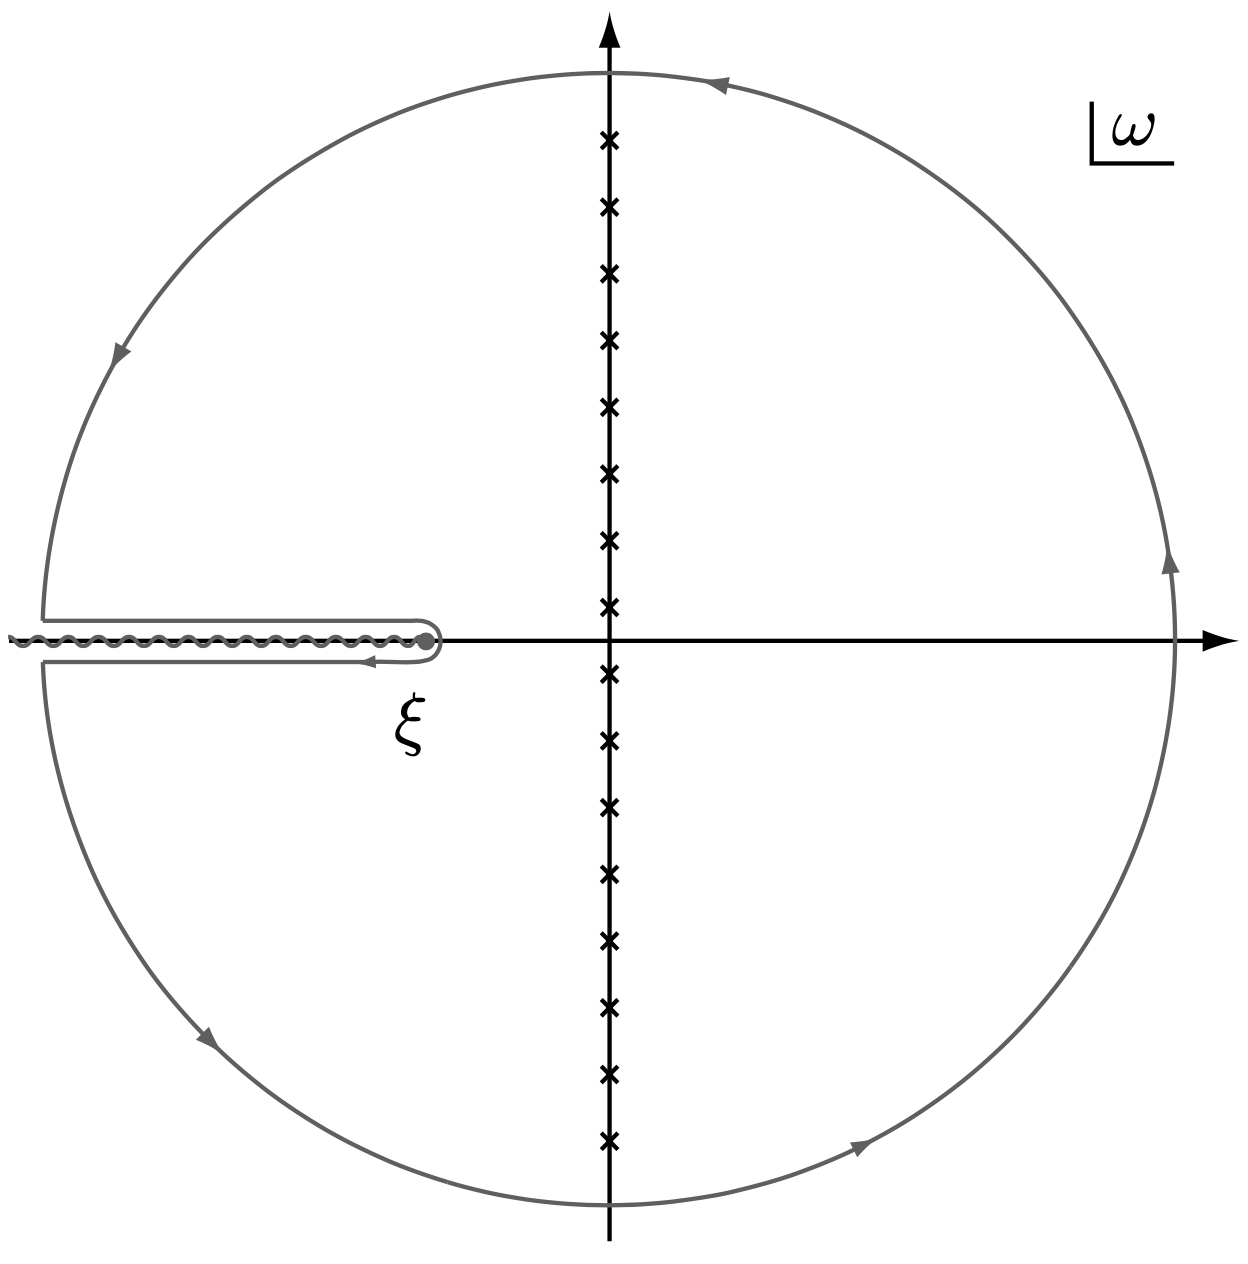
\includegraphics[width=0.25\linewidth]{pics/FqSum.png}
%\end{equation*}
The free energy is
\begin{equation}
\begin{aligned}
	F &= \frac{1}{2\pi i}\int_{-\infty}^\infty dx \rho(x)\ln\left(\frac{\xi-x-i\epsilon}{\xi-x+i\epsilon}\right) \\
	&= \frac{-\zeta}{2\pi i\beta} \int_{-\infty}^{\infty}dx \ln(1-\zeta e^{-\beta z})\left(\frac{1}{x+i\epsilon-\xi}-\frac{1}{x-i\epsilon-\xi}\right),
\end{aligned}
\end{equation}
where we integrate the expression by part, noticing that
\begin{equation}
	\frac{d}{dz} \frac{\zeta}{\beta} \ln(1-\zeta e^{-\beta z}) = \frac{1}{e^{\beta z}-\zeta} = \rho(z)
\end{equation}
Using the identity
\begin{equation*}
	\lim_{\epsilon\rightarrow 0^+} \frac{1}{x+i\epsilon} = -i\pi\delta(x) + \mathcal{P}\frac{1}{x},
\end{equation*}
the above expression can be simplified to
\begin{equation}
	F = \frac{\zeta}{\beta} \ln(1-\zeta e^{-\beta\zeta}).
\end{equation}






\section{Path Integral Formalism}

\subsection{Generating Functionals}
In this section, we are discussing general interacting field theory.
Consider the action for free field with source
\begin{equation}
	S[\phi,J]
	= \int d^dx\left[\mathcal{L}(\phi) + J(x)\cdot\phi(x) \right].
\end{equation}
In the path integral formalism, we consider the partition function with source:
\begin{equation}
	Z[J] = \int D[\phi]\ e^{iS[\phi,J]}.
\end{equation}
The central quantity a field theory produces is the correlation function of field values at different spacetime points:
\begin{equation}
	C(x_1,\cdots,x_n) \equiv \langle \phi(x_1)\cdots \phi(x_n)\rangle,
\end{equation}
where $\langle \cdots \rangle$ denotes the (time-ordered) average defined by the functional integral:
\begin{equation}
	\langle \cdots \rangle \equiv \frac{1}{Z[0]}\int D[\phi]\ e^{-iS[\phi]} (\cdots).
\end{equation}
We see that the partition function produce all possible correlation functions:
\begin{equation}
	C(x_1,\cdots,x_n) = \left. \prod_{i=1}^n \left[\frac{\delta}{i\delta J(x_i)}\right] Z[J] \right|_{J=0}.
\end{equation}
The partition function $Z[J]$ is thus a generating functional.
For interaction theory, the perturbation approach is that we first evaluate the generating functional for free field $Z_0[J]$, then the generating functional for interacting field can be formally expressed as:
\begin{equation}
	Z[J] = \exp\left(i\int d^dx \mathcal{L}_{\mathrm{int}}\left[\frac{\delta}{i\delta J(x)}\right]\right)Z_0[J],
\end{equation}
which can then be Taylor expanded order by order.
Since the unconnected diagram can be absorbed into $Z[0]$, we only need to calculate the connected diagram.
The procedure of perturbative expansion with only connected diagrams can be formally represented by introducing the quantity $Z[J] = Z[0]\exp\left(i W[J]\right)$.
The perturbative expansion of $W[J]$ contain only the connected diagrams.
Note that for the free theory,
\begin{equation*}
	\frac{Z_0[J]}{Z_0[0]} = \exp\left[-\frac{i}{2}\int d^d x_1 d^d x_2 J(x_1) \Delta(x_1-x_2)J(x_2)\right],
\end{equation*}
which means
\begin{equation*}
	W_0 = -\frac{1}{2}\int d^d x_1 d^d x_2 J(x_1) \Delta(x_1-x_2)J(x_2).
\end{equation*}

Consider the four-point connected correlation:
\begin{equation}
	iV_4 \equiv \langle \mathcal{T}\phi(x_1) \phi(x_2) \phi(x_3) \phi(x_4)\rangle_c
\end{equation}
Following the same procedure,
\begin{equation}
\begin{aligned}
	iV_4 
	=&\ i\left.\frac{\delta^4 W[J]}{i\delta J(x_1)i\delta J(x_2)i\delta J(x_3)i\delta J(x_4)}\right|_{J=0} \\
	=&\ \frac{1}{Z[0]}\left.\frac{\delta^4 Z[J]}{i\delta J(x_1)i\delta J(x_2)i\delta J(x_3)i\delta J(x_4)}\right|_{J=0} \\
	&-i\Delta(x_1-x_2) i\Delta(x_3-x_4) -i\Delta(x_1-x_3) i\Delta(x_2-x_4) -i\Delta(x_1-x_4) i\Delta(x_2-x_3).
\end{aligned}
\end{equation}
The connected correlation function automatically omit those disconnected components.

\subsection{Free Scalar Field}

Now we evaluate the propagator in the path-integral formalism.
In momentum space, the free action (with source) is 
\begin{equation*}
	\frac{1}{V}\sum_k \left[\frac{1}{2}\tilde\phi^*(k)( k^2-m^2)\tilde\phi(k)+\tilde J^*(k)\cdot\tilde\phi(k)+\tilde\phi^*(k)\cdot\tilde J(k)\right].
\end{equation*}
For real field, $\tilde\phi^*(k) = \tilde\phi(-k)$.
For our convenience, we have expressed the momentum integral as summation.
Actually, consider the $d$-dimensional box of size $L^d$, the momentum along each axis is multiple of $2\pi/L$, so when $L\rightarrow \infty$, the summation approaches in integral,
\begin{equation*}
	\frac{1}{V}\sum_k \rightarrow \int \frac{d^d k}{(2\pi)^d}.
\end{equation*}
Let us omit the $1/V$ factor, the summation can be formally expressed as
\begin{equation}
	\frac{1}{4}\mathbf{v}^T \cdot \mathbf M\cdot \mathbf{v} + \frac{1}{2}\mathbf{j}^T \cdot \mathbf{v}
\end{equation}
where
\begin{equation*}
	\mathbf v = \bigoplus_{|\mathbf k|} \left[
	\begin{array}{c}
		\tilde{\phi}(k) \\ 
		\tilde{\phi}^*(k) 
	\end{array}\right],\ 
	\mathbf M = \bigoplus_{|\mathbf k|} \left[
	\begin{array}{cc} 
		0 & k^2-m^2 \\ 
		k^2-m^2 & 0 
	\end{array}\right],\ 
	\mathbf j = \bigoplus_{|\mathbf k|} \left[
	\begin{array}{c}
		\tilde{J}^*(k) \\ 
		\tilde{J}(k) 
	\end{array}\right].
\end{equation*}
Note that in the above expression, we have made an infinitesimal shift of mass ($m^2 \rightarrow m^2 - i\epsilon$) to ensure the convergence of the Gaussian integral.
The integrated variables $v_i$ is not real.
To use the real Gaussian integral formula, we make use of a unitary transformation: 
\begin{equation*}
	\mathbf U = \frac{1}{\sqrt 2} \left[\begin{array}{cc}
		1 & 1 \\
		-i & i
	\end{array}\right], \quad
	\mathbf U \cdot \left[
	\begin{array}{c}
		\tilde{\phi}(k) \\ 
		\tilde{\phi}^*(k) 
	\end{array}\right] 
	= \frac{1}{\sqrt 2}\left[
	\begin{array}{c}
		\tilde\phi(k)+\tilde\phi^*(k) \\ 
		-i\tilde\phi(k)+i\tilde\phi^*(k)
	\end{array}\right]
	\equiv \left[
	\begin{array}{c}
		\tilde\phi_1(k) \\ 
		\tilde\phi_2(k) 
	\end{array}\right]
\end{equation*}
The path integral then becomes a real field integral.
Recall the real Gaussian integral formula:
\begin{equation}
	\int d\mathbf x \exp\left(-\frac{1}{2}\mathbf{x}^T \cdot \mathbf A \cdot \mathbf{x} + \mathbf{B}^T \cdot \mathbf{x}\right) 
	= \sqrt{\frac{(2\pi)^N}{\det{\mathbf A}}}\exp\left(\frac{1}{2}\mathbf{B}^T \cdot \mathbf{A}^{-1} \cdot \mathbf{B}\right),
	\label{eq:real-gaussian-integral}
\end{equation}
For the field integral, we absorbed the $(2\pi)^{N/2}$ term into the measure, and express the path integral for the Gaussian field as:
\begin{equation}
	W_0[J] 
	= -\frac{i}{4}\int \frac{d^d k}{(2\pi)^d} \mathbf j^T_k \cdot \mathbf M^{-1}_k \cdot \mathbf j_k
	= -\frac{1}{2} \int \frac{d^d k}{(2\pi)^d}  \tilde{J}^*(k) \tilde{\Delta}_0(k) \tilde{J}(k).
\end{equation}
This gives the propagator in the momentum space:
\begin{equation}
	\tilde{\Delta}_0(k) = \frac{i}{k^2-m^2}
	\quad \Longrightarrow \quad 
	\Delta_0(x_1-x_2) = i\int\frac{d^{4} k}{(2\pi)^{4}} \frac{e^{-i k\cdot (x_1-x_2)}}{k^2-m^2}.
\end{equation}


\subsection{From Field to Force}
Consider two separate particle described by the delta function $J_a(x) = \delta^{(3)}(\bm x - \bm x_a)$, together the source is
\begin{equation}
	J(x) = J_1(x) + J_2(x).
\end{equation}
Adding the source,
\begin{equation*}
	W_0[J] = -\frac{1}{2}\int d^4x_1 d^4 x_2 J(x_1) \Delta_0(x_1-x_2) J(x_2)
\end{equation*}
Omit the self energy terms $J_1^2(x), J_2^2(x)$, $W_0[J]$ is
\begin{equation}
\begin{aligned}
	W_0[J] &= -\int d^4 y_1 d^4 y_2\ e^{-ik^0(y_1^0-y_2^0)}\int \frac{d^4 k}{(2\pi)^4} J_1(y_1)\frac{e^{i\bm k\cdot (\bm y_1-\bm y_2)}}{k^2-m^2} J_2(y_2) \\
	&= -\int  dt \int d (y_1^0 - y_2^0) \ e^{-ik^0(y_1^0-y_2^0)}\int \frac{d^4 k}{(2\pi)^4} \frac{e^{i\bm k\cdot (\bm y_1-\bm y_2)}}{k^2-m^2} \\
	&= \left(\int dt \right)\int \frac{d^3 k}{(2\pi)^3} \frac{e^{i\bm k\cdot (\bm y_1-\bm y_2)}}{\bm k^2 + m^2}
\end{aligned}
\end{equation}
Recall that the partition function is actually infinite:
\begin{equation}
	Z_0 \sim \langle 0| e^{-i H_0 T} |0\rangle \quad \Longrightarrow \quad
	W_0 = -i E T,
\end{equation}
where $E$ is the energy.
Writing $\bm r \equiv \bm y_1 - \bm y_2$, and $u \equiv \cos\theta$ with $\theta$ the angle between $\bm k$ and $\bm r$, the volume form is $dk \cdot kd\theta \cdot  2\pi k \sin \theta = 2\pi k^2 dk du$, and the integral is
\begin{equation}
\begin{aligned}
	E &= -\int \frac{d^3 k}{(2\pi)^3} \frac{e^{i k r u}}{k^2 + m^2} \\
	&= - \frac{1}{(2\pi)^2} \int_0^\infty k^2 dk \int_{-1}^1 du \frac{e^{ikru}}{k^2 +m^2} \\
	&= -\frac{1}{2\pi^2 r} \int_0^\infty k  \frac{\sin kr}{k^2 +m^2} dk.
\end{aligned}
\end{equation}
Since the integral is even, we can extend the integral to
\begin{equation}
\begin{aligned}
	E &= -\frac{1}{4\pi^2 r} \int_{-\infty}^\infty k  \frac{\sin kr}{k^2 +m^2} dk \\
	&= \frac{i}{4\pi^2 r} \int_{-\infty}^\infty \frac{k e^{ikr}}{k^2 +m^2} dk
\end{aligned}
\end{equation}
The residue theorem gives
\begin{equation}
	\int_{-\infty}^\infty \frac{k e^{ikr}}{k^2 +m^2} dk = \pi ie^{-mr}
\end{equation}
So we get the potential of two particles:
\begin{equation}\label{eq:field-to-force}
	V(r) = -\frac{e^{-mr}}{4\pi r},
\end{equation}
and the attractive force is
\begin{equation}
	F(r) = -\frac{dV}{dr} = -(1+mr)\frac{e^{-mr}}{4\pi r^2}.
\end{equation}
We see that in the massless case, the force gives the long-range Coulomb force $F \propto 1/r^2$, while in the massive field theory, the force is short-ranged, with the decay length proportional to the mass.


\subsection{Symmetries}

A (classical) symmetry means that the equation of motion dictated by a Lagrangian is invariant under the (usually infinitesimal) transformation (denoted as $\Lambda$, but not necessarily the Lorentz transformation), the coordinate and the field transform as
\begin{equation}
\begin{aligned}
	x^\mu &\rightarrow {x'}^\mu = x^\mu + \omega_a \frac{\delta x^\mu}{\delta \omega_a}, \\
	\phi(x) &\rightarrow \phi'(x') = \phi(x) + \omega_a \frac{\delta \mathcal F}{\delta \omega_a}(x).
\end{aligned}
\end{equation}
Here the field $\phi$ may contain additional internal degrees of freedom. 
Also here we adopt the active view of the field transformation, meaning that for a fixed coordinate $x$, the transformation of the field is
\begin{equation}
	\delta_\omega \phi(x) \equiv \phi'(x) - \phi(x) = - i\omega_a \hat G_a \phi(x),
\end{equation}
where by comparing the definitions, we know
\begin{equation}
	\hat G_a\phi(x) = \frac{\delta x^\mu}{\delta\omega_a} \partial_\mu \phi(x) - \frac{\delta\mathcal F}{\delta\omega_a}.
\end{equation}

\subsubsection{Noether's Theorem}
The action under the above transformation becomes
\begin{equation}
	S' = \int d^d x' \mathcal L\left(\phi'(x'),\frac{\partial \phi'}{\partial {x'}^\mu}(x')\right).
\end{equation}
We are going to expand the expression to the first order of $\omega_a$'s.
Note that there are two contributions to the change of action: one from the coordinate change and the other from the Lagrangian.
For the coordinate part, we have
\begin{equation}
	\frac{\partial {x'}^\mu}{\partial x^\nu}
	= \delta^\mu_\nu + \partial_\nu\left(\omega_a \frac{\delta x^\mu}{\delta \omega_a}\right).
\end{equation}
Using the relation 
\begin{equation}
	\det(1+E) = 1 + \Tr E, \quad E\text{ small},
\end{equation}
we know by changing the variable $x' \rightarrow x$, we get a contribution
\begin{equation}
\begin{aligned}
	\delta S 
	&= \int d^d x \left|\det \frac{\partial {x'}^\mu}{\partial x^\nu}\right|\left(\mathcal L + \omega_a \frac{\delta x^\mu}{\delta \omega_a} \partial_\mu \mathcal L \right)  \\
	&= \int d^d x \ \partial_\mu \left(\mathcal L \omega_a \frac{\delta x^\mu}{\delta \omega_a}\right).
\end{aligned}
\end{equation}
On the other hand, the change of Lagrangian is
\begin{equation}
	{\delta} \mathcal L =
	\left[\frac{\partial \mathcal L}{\partial \phi} -\partial_\mu \frac{\partial\mathcal L}{\partial(\partial_\mu\phi)} \right]\delta_\omega \phi + \partial_\mu \left(\frac{\partial\mathcal L}{\partial(\partial_\mu\phi)} \delta_\omega \phi \right).
\end{equation}
The first term vanishes as the result of classical EOM.
Together, the change of action is
\begin{equation}
\begin{aligned}
	\delta S 
	&= \int d^d x \ \partial_\mu \left(\mathcal L \omega_a \frac{\delta x^\mu}{\delta \omega_a}+\frac{\partial\mathcal L}{\partial(\partial_\mu\phi)} \delta_\omega \phi \right) \\
	&= \int d^d x \ \partial_\mu \left[\left(\delta^\mu_\nu \mathcal L - \frac{\partial\mathcal L}{\partial(\partial_\mu\phi)}\partial_\nu \phi(x) \right)\frac{\delta x^\nu}{\delta\omega_a}  + \frac{\partial\mathcal L}{\partial(\partial_\mu\phi)}\frac{\delta\mathcal F}{\delta\omega_a}\right] \omega_a \\
	&\equiv \int d^d x \ \omega_a  \partial_\mu J^\mu_a.
\end{aligned} 
\end{equation}
The symmetry requires that the action is invariant over arbitrary spacetime region, so that $J_a^\mu$ is conserved current.
Note that we can freely add a derivative of an anti-symmetric tensor to the current:
\begin{equation}
	J^\mu_a \rightarrow J^\mu_a + \partial_\nu B^{\nu\mu}_a,\quad
	B^{\mu\nu} = -B^{\nu\mu}.
\end{equation}
The above discussion gives the Noether's theorem, which says that symmetries in classical field theory imply conserved quantities.

\subsubsection{Ward Identity}
The quantum version of the Noether's theorem is the Ward identity.
From the above discussion, we consider a \textit{local} transformation, i.e., $\omega_a(x)$ now depend on coordinate $x$.
The action under such transformation becomes:
\begin{equation}
\begin{aligned}
	S &\rightarrow \int d^d x \left[\mathcal L(x) + \partial_\mu\left( \omega_a(x) J_a^\mu \right) + \omega_a(x) F_a(x)\right] \\
	&= \int d^d x \left[\mathcal L(x) + \omega_a(x) \partial_\mu J_a^\mu + \omega_a(x) (F_a+\partial_\mu J^\mu)\right],
\end{aligned}
\end{equation}
where $\omega_a(x) F_a(x)$ comes from the classical EOM term that no longer vanishes automatically.
However, using the fact that when $\omega_a(x)$ is constant, the action is invariant (over arbitrary region), any term involving $\omega(x)$ should be zero. 
We thus know the action only depend on the derivative of $\omega_a(x)$, i.e.,
\begin{equation}
	S \rightarrow \int d^d x \left[\mathcal L(x) + J_a^\mu \partial_\mu \omega_a(x)  \right],
\end{equation}
Consider the quantum partition function $Z = \int D[\phi] e^{iS[\phi]}$.
After the infinitesimal transformation, the partition function becomes
\begin{equation}
	Z = \int D[\phi'] e^{iS[\phi]} \exp\left[-i\int d^d x \ \omega_a(x) \partial_\mu J_a^\mu (x)\right].
\end{equation}
Note that the infinitesimal transformation for path-integral is nothing but a change of variable.
If we assume the transformation does not change the measure: $D[\phi'] = D[\phi]$, then the quantum partition function is invariant under the local transformation.
This implies the operator identity:
\begin{equation}
	\partial_\mu J_a^\mu(x) = 0.
\end{equation}
Note that the operator identity should be understood as a set of identity for correlation function.
Consider the generating functional $Z[K] =\int D[\phi] \exp(iS[\phi]+ i \int d^d x K \phi)$, where we denote the auxiliary current as $K$ to avoid confusion with conserved current.
For arbitrary infinitesimal (local) symmetry transformation, the generating functional
\begin{equation}
	Z[K] = \int D[\phi] e^{iS[\phi]+ i \int d^d x K \phi} \left[1-i\int d^d x\ \omega_a(x)\left(\partial_\mu J^\mu + K \hat G \phi \right) \right]
\end{equation}
remains the same, which means
\begin{equation}
	\int D[\phi] e^{iS[\phi]+ i \int d^d x K \phi} \left(\partial_\mu J^\mu(x) + K(x) \hat G \phi(x) \right) = 0.
\end{equation}
By taking derivative on $K(x_i)$ for $n$ times, and then set $K=0$, we get the Ward identity:
\begin{equation}
	\partial_\mu \langle J_a^\mu(x) \phi(x_1) \cdots \phi(x_n)\rangle = -i\delta(x-x_i) \sum_{i=1}^n \langle \phi_1 \cdots \hat G\phi(x_i)\cdots \phi_n\rangle.
\end{equation}
The right-hand side can be viewed as the contact due to the time-ordering;
It vanishes if $x \ne x_i$ for all $i$'s. 





\end{document}


